%%
%% 19May2008part1.tex
%% 
%% Made by Alex Nelson
%% Login   <alex@tomato>
%% 
%% Started on  Fri Dec 26 19:24:57 2008 Alex Nelson
%% Last update Fri Dec 26 19:24:57 2008 Alex Nelson
%%
\begin{ex}
%% \begin{figure}
%% \subfigure[Plot of $f$, $g$]{\label{img:19May2008:img1}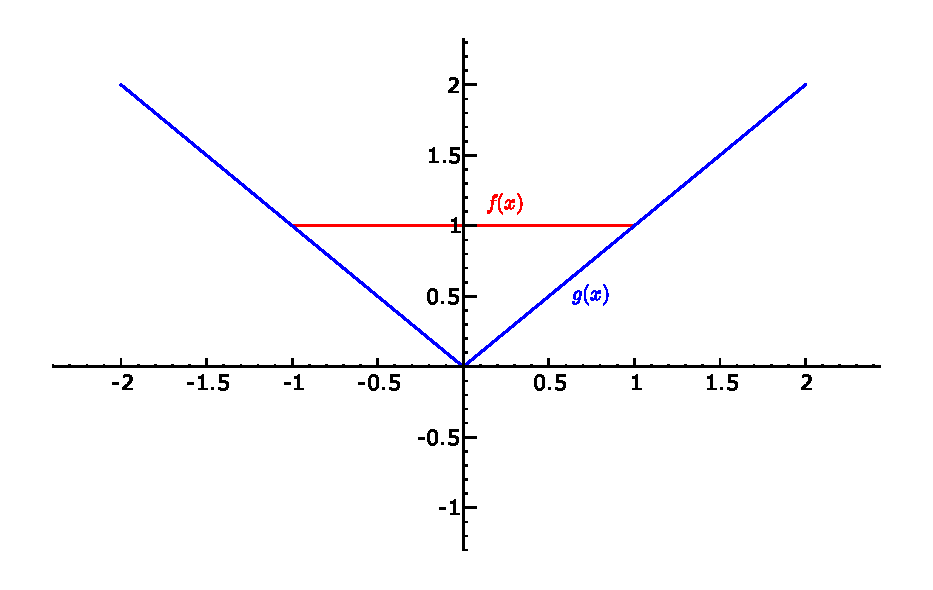
\includegraphics[width=0.3\textwidth]{img/19May2008img1.eps}}
%% \subfigure[When $1\leq x\leq3$]{\label{img:19May2008:img2}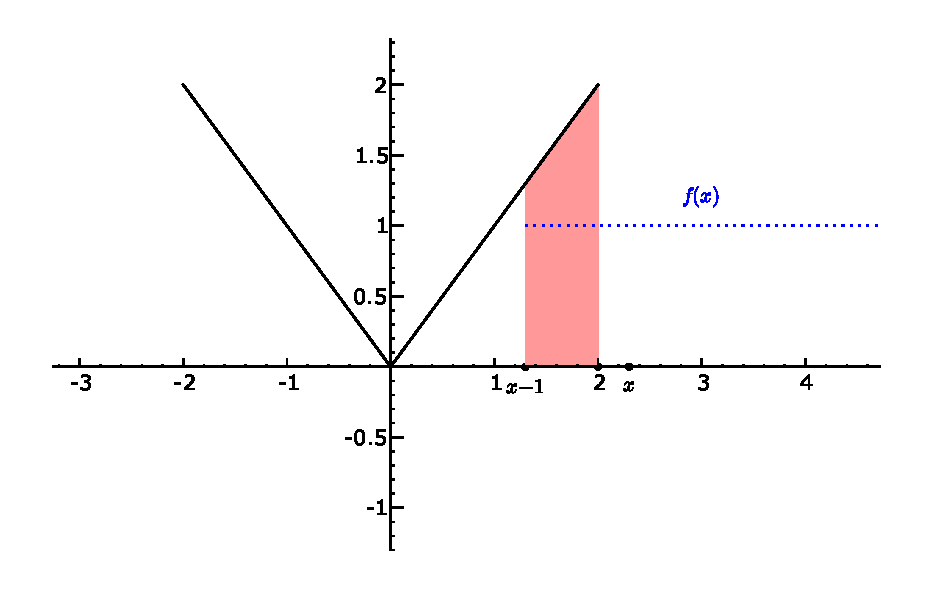
\includegraphics[width=0.3\textwidth]{img/19May2008img2.eps}}
%% \subfigure[When $0\leq x\leq 1$]{\label{img:19May2008:img3}\ingludegraphics[width=0.3\textwidth]{img/19May2008img3.eps}}
%% \end{figure}
\begin{figure}[ht!]
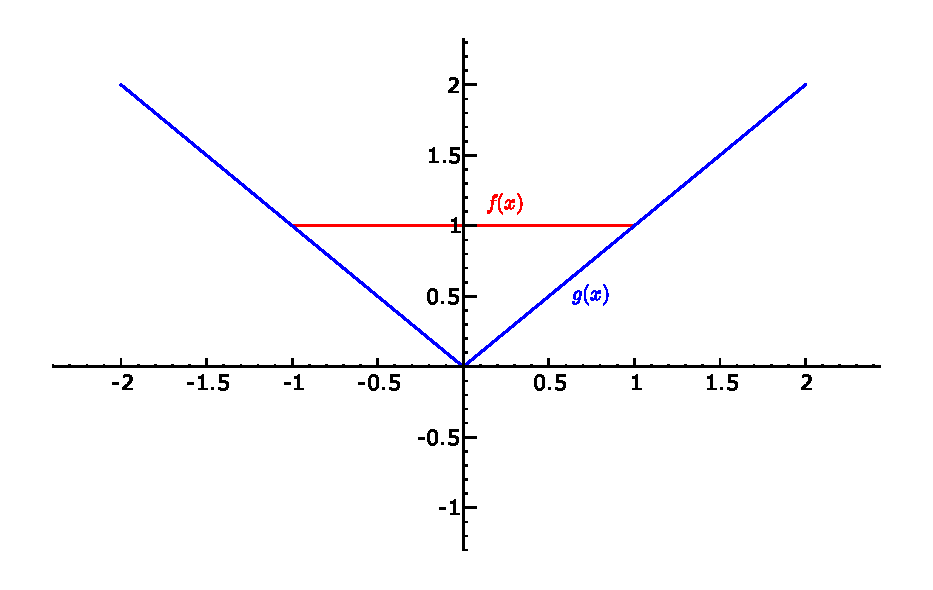
\includegraphics[width=\textwidth]{img/19May2008img1.eps}
\caption{Plot of $f$ and $g$}
\end{figure}
\begin{figure}[hb!]
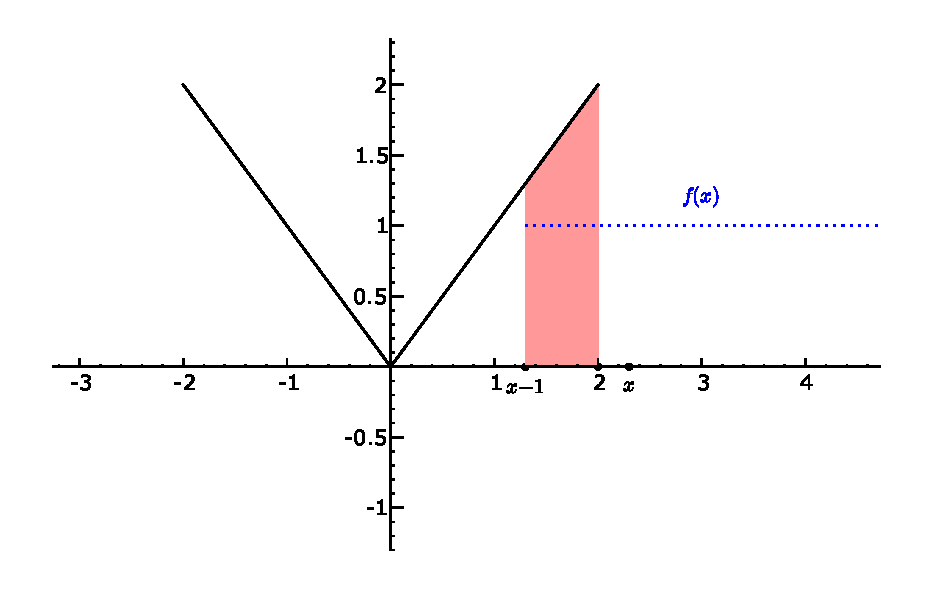
\includegraphics[width=\textwidth]{img/19May2008img2.eps}
\caption{When $1\leq x\leq3$}\label{img:19May2008:img2}
\end{figure}
Let
\begin{equation*}
f(x) = \begin{cases}1 &\text{when }|x|\leq1\\
0&\text{otherwise}\end{cases}
\end{equation*}
\begin{equation*}
g(x) = \begin{cases}|x| &\text{when }|x|\leq2\\
0&\text{otherwise}\end{cases}
\end{equation*}
Let us compute $\mathcal{F}[f*g]$.

\textbf{Direct Computation:} We see that we only really need
to compute the convolution for $x\geq0$ because both $f$ and
$g$ are even functions, so $(f*g)$ is also even. We can see
this assertion by
\begin{align*}
(f*g)(-x) &= \int f(y)g(-x-y)dy,\quad\text{let }z=-y\\
&= \int f(-z)g(-x+z)dz\\
&= \int f(z)g(x-z)dz\\
&= (f*g)(x)
\end{align*}
which is justified by the even-ness of $f$ and $g$. We also
see that when $x>3$, $(f*g)(x)=0$.
When $1\leq x\leq 3$, we see that
\begin{equation}
(f*g)(x) = \int^{2}_{x-1}ydy = \frac{1}{2}(4-(x-1)^2)
\end{equation}
by direct computation. The integral is shown in figure \eqref{img:19May2008:img2}.

For $0\leq x\leq 1$, we have
\begin{subequations}
\begin{align}
(f*g)(x) &= \int^{0}_{x-1}ydy + \int^{x+1}_{0}ydy\\
&= \frac{-1}{2}y^2\Big|^{0}_{x-1} +
  \frac{1}{2}y^2\Big|^{x+1}_{0}\\
&= x^2 + 1.
\end{align}
\end{subequations}
The integral is doodled in figure \eqref{img:19May2008:img3}.
\begin{figure}[hb!]
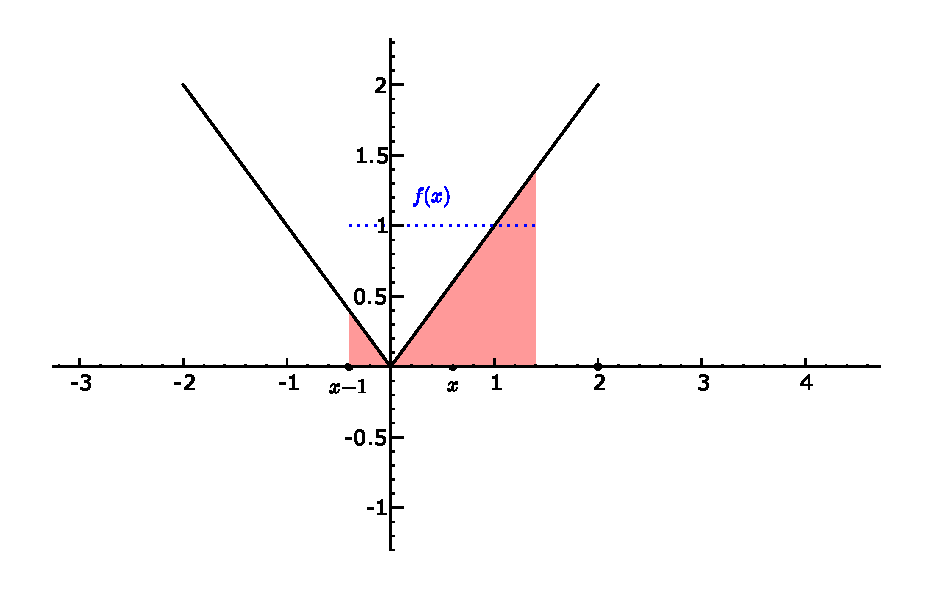
\includegraphics[width=\textwidth]{img/19May2008img3.eps}
\caption{For $0\leq x\leq 1$}\label{img:19May2008:img3}
\end{figure}

We then find
\begin{equation}
(f*g)(x) = \begin{cases} x^2+1, &|x|\leq1\\
2 - \frac{1}{2}(|x|-1)^2, & 1\leq|x|\leq3\\
0 &\text{otherwise}.
\end{cases}
\end{equation}
The Fourier transform is then
\begin{equation}
\mathcal{F}[(f*g)] = \int^{1}_{-1}( x^2+1)e^{-i\xi x}dx + \int_{1\leq|x|\leq3}(2
- \frac{1}{2}(|x|-1)^2)e^{-i\xi x}dx
\end{equation}
This is a bit of a difficult thing to evaluate, so perhaps
we shouldn't even try.

On the other hand, we can find
\begin{equation}
\mathcal{F}[f] = \widehat{f}(\xi) = 2\frac{\sin(\xi)}{\xi}
\end{equation}
and similarly
\begin{subequations}
\begin{align}
\int^{A}_{0}xe^{-i\xi x}dx &= \frac{ix}{\xi}e^{-i\xi
  x}\Big|^{A}_{0} - \frac{i}{\xi}\int^{A}_{0}e^{-i\xi x}dx\\
&= \frac{iA}{\xi}e^{-iA\xi} - \frac{1}{\xi^2} + \frac{1}{\xi^2}e^{-iA\xi}\\
&= \left(\frac{1}{\xi^2} + \frac{iA}{\xi}\right)e^{-iA\xi} - \frac{1}{\xi^2}\\ 
\mathcal{F}[g] &= \int^{2}_{0}xe^{-i\xi x}dx -\int^{0}_{-2}xe^{-i \xi x}dx\\ 
&= \int^{2}_{0}xe^{-i\xi x}dx +\int^{-2}_{0}xe^{-i \xi x}dx\\ 
&= \left(\frac{1}{\xi^2}+\frac{i2}{\xi}\right)e^{-i2\xi} +
\left(\frac{1}{\xi^2} - \frac{i2}{\xi}\right)e^{i2\xi} -
\frac{2}{\xi^2}\\
&= \frac{2\cos(2\xi)}{\xi^2} + \frac{4\sin(2\xi)}{\xi} - \frac{2}{\xi^2}
\end{align}
\end{subequations}
Thus
\begin{equation}
\mathcal{F}[f*g] = \widehat{f}(\xi)\widehat{g}(\xi) =
  \left(2\frac{\sin(\xi)}{\xi}\right)\left[\frac{2\cos(2\xi)}{\xi^2} + \frac{4\sin(2\xi)}{\xi} - \frac{2}{\xi^2}\right]
\end{equation}
which would have been an impossible integral to perform if
we did it the direct, naive way.
\end{ex}
\subsection{Applications of the Fourier Transform}

\marginpar{Applications: Differential Equations}One of the most useful applications of the Fourier transform
is to solve differential equations. Usually, it is on
unbounded domains. What does this mean? Well, if the
function has boundaries of $(-\infty,\infty)$, or
$(-\infty,0)$, or $(0,\infty)$, then it's domain is
unbounded.\index{Fourier Transform!Solving Differential Equations}

\begin{ex}{(Heat Equation)}\index{Heat Equation!Solved Using Fourier Transform}
The heat equation is
\begin{equation}
\partial_{t}u(x,t) =
k\partial_{x}^{2}u(x,t),\quad-\infty\leq x\leq\infty.
\end{equation}
There is no boundary condition for $u$ but we have the
initial condition $u(x,0)=f(x)$. We can take the Fourier
transform in the $x$ variable to find
\begin{equation}
\partial_{t}\widehat{u}(\xi,t) = k(i\xi)^2\widehat{u}(\xi,t)
= -k\xi^{2}u(\xi,t)
\end{equation}
This is a first order differential equation in time, which
has the solution
\begin{equation}
\widehat{u}(\xi,t) = \widehat{f}(\xi)e^{-k\xi^2t}
\end{equation}
If we define
\begin{equation}
K_{t}(x) = \mathcal{F}^{-1}[e^{-k\xi^2t}] =
\frac{1}{\sqrt{4\pi kt}}e^{-x^2/(4kt)}
\end{equation}
(where we just used our relation of the Fourier transform of
the Gaussian to justify this), then
\begin{equation}
\widehat{u}(\xi,t) = \mathcal{F}[f*K_{t}]
\end{equation}
thus
\begin{equation}
u(x,t) = (f*K_{t})(x) = \frac{1}{\sqrt{4\pi kt}}\int f(y)e^{-(x-y)^{2}/4kt}dy.
\end{equation}
\end{ex}
\begin{ex}{(Wave Equation)}\index{Wave Equation!Solve With Fourier Transform}
The wave equation for an unbounded wave is
\begin{equation}
\partial_{x}^{2}u(x,y) + \partial_{y}^{2}u(x,y) = 0,\quad
-\infty<x<\infty,\quad y>0
\end{equation}
We would like to look for bounded solutions. So we take the
Fourier transform in $x$ and find
\begin{equation}
-\xi^2\widehat{u}+\partial_{y}^{2}\widehat{u} = 0
\end{equation}
The initial condition becomes
$\widehat{u}(\xi,0)=\widehat{f}(\xi)$. So we've changed the
wave equation into a second order ODE, the characteristic
equation is
\begin{equation}
-\xi^2 + r^2 = 0\Rightarrow r=\pm|\xi|.
\end{equation}
So, the general solution is
\begin{equation}
\widehat{u}(\xi,y) = c_{1}(\xi)e^{|\xi|y} + c_{2}(\xi)e^{-|\xi|y}
\end{equation}
Observe that as $\xi\to\pm\infty$, the first term goes to
infinity. So, due to our demand of making $u$ bounded, we
need to set $c_1=0$. Thus our solution becomes (by imposing
our initial condition)
\begin{subequations}
\begin{align}
\widehat{u}(\xi,y) &= c_{2}(\xi)e^{-|\xi|y}\\
&= \widehat{f}(\xi)e^{-|\xi|y}.
\end{align}
\end{subequations}
Once again, this is a Fourier transform of $f$ convoluted
with some function. We then write
\begin{equation}
\widehat{u}(\xi,y) = \widehat{f}(\xi)e^{-|\xi|y} = \mathcal{F}[f*P_y]
\end{equation}
so we define
\begin{equation}
P_{y}(x) = \mathcal{F}^{-1}[e^{-|\xi|y}]
\end{equation}
which is a special function. We call it the \textbf{Poisson Kernel}\index{Poisson Kernel}
and we can write it out explicitly as
\begin{equation}
  \addtolength{\fboxsep}{5pt}
   \boxed{
   \begin{gathered}
     P_{y}(x) = \frac{y}{\pi(x^2+y^2)}.
   \end{gathered}
   }
\end{equation}
We can now write the general solution of the wave equation
as
\begin{equation}
u(x,y) = (f*P_y)(x) = \int\frac{yf(x-y)}{\pi(x^2+y^2)}dy.
\end{equation}
This concludes our example.
\end{ex}

\marginpar{Applications: Signal Analysis}The other application is signal analysis. We represent a
signal as a function of time, $f(t)$, representing the
amplitude of a signal at time $t$ (e.g. a sound signal,
$f(t)$ would be the volume of the sound, etc.).

By the Fourier inversion formula
\begin{equation}
f(t) = \frac{1}{2\pi}\int e^{i\omega
  t}\widehat{f}(\omega)d\omega
\end{equation}
where $\widehat{f}(\omega)$ is the Fourier transform
\begin{equation}
\widehat{f}(\omega) = \int f(t)e^{-i\omega t}dt
\end{equation}
where $t$ is time, and $\omega$ is frequency; we have $t$ in
units of (e.g) seconds, and $\omega$ in units of Herz
(``cycles per second'').

The Fourier inversion represents $f(t)$ as a (continuous) superposition
of periodic and simple waves. That is
\begin{equation}
e^{i\omega t} = \text{ periodic simple waves}
\end{equation}
and
\begin{equation}
\mathcal{F}^{-1}[\widehat{f}(\omega)] = \begin{pmatrix}
$representation$\ $of$\ f(t)\ $as$\\
$continuous$\ $superposition$\ $of$\\
$simple$\ $periodic$\ $waves$.
\end{pmatrix}.
\end{equation}

We also model systems (e.g. an electrical system, or a
telephone system) with an operator $L$
\begin{align*}
L:&f\to L[f]\\
&\text{input}\to\text{output}
\end{align*}
When $L$ is linear, we have a linear system. If $L$ is
shift-invariant, then $L$ commutes with translations. What
do we mean by this? Well, if
\begin{equation}
L[f(x)]=g(x)\Rightarrow L[f(x+k)] = g(x+k)
\end{equation}
for some arbitrary constant $k$, then an operator that
shifts $f$ by 1
\begin{equation}
E[f(x)] = f(x+1)
\end{equation}
can be interchanged with $L$:
\begin{equation}
L[E[f(x)]]=E[L[f(x)]].
\end{equation}
For instance, the AM radio operator is a linear, shift
invariant system. 
